\documentclass[journal,12pt,twocolumn]{IEEEtran}
\usepackage{setspace}
\usepackage{gensymb}
\usepackage{caption}
%\usepackage{multirow}
%\usepackage{multicolumn}
%\usepackage{subcaption}
%\doublespacing
\singlespacing
\usepackage{csvsimple}
\usepackage{amsmath}
\usepackage{multicol}
%\usepackage{enumerate}
\usepackage{amssymb}
%\usepackage{graphicx}
\usepackage{newfloat}
%\usepackage{syntax}
\usepackage{listings}
\usepackage{color}
\usepackage{tikz}
\usepackage{graphicx}
\usetikzlibrary{shapes,arrows}

%\usepackage{graphicx}
%\usepackage{amssymb}
%\usepackage{relsize}
%\usepackage[cmex10]{amsmath}
%\usepackage{mathtools}
%\usepackage{amsthm}
%\interdisplaylinepenalty=2500
%\savesymbol{iint}
%\usepackage{txfonts}
%\restoresymbol{TXF}{iint}
%\usepackage{wasysym}
\usepackage{amsthm}
\usepackage{mathrsfs}
\usepackage{txfonts}
\usepackage{stfloats}
\usepackage{cite}
\usepackage{cases}
\usepackage{mathtools}
\usepackage{caption}
\usepackage{enumerate}	
\usepackage{enumitem}
\usepackage{amsmath}
%\usepackage{xtab}
\usepackage{longtable}
\usepackage{multirow}
%\usepackage{algorithm}
%\usepackage{algpseudocode}
\usepackage{enumitem}
\usepackage{mathtools}
\usepackage{hyperref}
%\usepackage[framemethod=tikz]{mdframed}
\usepackage{listings}
    %\usepackage[latin1]{inputenc}                                 %%
    \usepackage{color}                                            %%
    \usepackage{array}                                            %%
    \usepackage{longtable}                                        %%
    \usepackage{calc}                                             %%
    \usepackage{multirow}                                         %%
    \usepackage{hhline}                                           %%
    \usepackage{ifthen}                                           %%
  %optionally (for landscape tables embedded in another document): %%
    \usepackage{lscape}     


\usepackage{url}
\def\UrlBreaks{\do\/\do-}


%\usepackage{stmaryrd}


%\usepackage{wasysym}
%\newcounter{MYtempeqncnt}
\DeclareMathOperator*{\Res}{Res}
%\renewcommand{\baselinestretch}{2}
\renewcommand\thesection{\arabic{section}}
\renewcommand\thesubsection{\thesection.\arabic{subsection}}
\renewcommand\thesubsubsection{\thesubsection.\arabic{subsubsection}}

\renewcommand\thesectiondis{\arabic{section}}
\renewcommand\thesubsectiondis{\thesectiondis.\arabic{subsection}}
\renewcommand\thesubsubsectiondis{\thesubsectiondis.\arabic{subsubsection}}

% correct bad hyphenation here
\hyphenation{op-tical net-works semi-conduc-tor}

%\lstset{
%language=C,
%frame=single, 
%breaklines=true
%}

%\lstset{
	%%basicstyle=\small\ttfamily\bfseries,
	%%numberstyle=\small\ttfamily,
	%language=Octave,
	%backgroundcolor=\color{white},
	%%frame=single,
	%%keywordstyle=\bfseries,
	%%breaklines=true,
	%%showstringspaces=false,
	%%xleftmargin=-10mm,
	%%aboveskip=-1mm,
	%%belowskip=0mm
%}

%\surroundwithmdframed[width=\columnwidth]{lstlisting}
\def\inputGnumericTable{}                                 %%
\lstset{
%language=C,
frame=single, 
breaklines=true,
columns=fullflexible
}

\begin{document}
%
\tikzstyle{block} = [rectangle, draw,
    text width=3em, text centered, minimum height=3em]
\tikzstyle{sum} = [draw, circle, node distance=3cm]
\tikzstyle{input} = [coordinate]
\tikzstyle{output} = [coordinate]
\tikzstyle{pinstyle} = [pin edge={to-,thin,black}]

\theoremstyle{definition}
\newtheorem{theorem}{Theorem}[section]
\newtheorem{problem}{Problem}
\newtheorem{proposition}{Proposition}[section]
\newtheorem{lemma}{Lemma}[section]
\newtheorem{corollary}[theorem]{Corollary}
\newtheorem{example}{Example}[section]
\newtheorem{definition}{Definition}[section]
%\newtheorem{algorithm}{Algorithm}[section]
%\newtheorem{cor}{Corollary}
\newcommand{\BEQA}{\begin{eqnarray}}
\newcommand{\EEQA}{\end{eqnarray}}
\newcommand{\define}{\stackrel{\triangle}{=}}
\bibliographystyle{IEEEtran}
%\bibliographystyle{ieeetr}
\providecommand{\nCr}[2]{\,^{#1}C_{#2}} % nCr
\providecommand{\nPr}[2]{\,^{#1}P_{#2}} % nPr
\providecommand{\mbf}{\mathbf}
\providecommand{\pr}[1]{\ensuremath{\Pr\left(#1\right)}}
\providecommand{\qfunc}[1]{\ensuremath{Q\left(#1\right)}}
\providecommand{\sbrak}[1]{\ensuremath{{}\left[#1\right]}}
\providecommand{\lsbrak}[1]{\ensuremath{{}\left[#1\right.}}
\providecommand{\rsbrak}[1]{\ensuremath{{}\left.#1\right]}}
\providecommand{\brak}[1]{\ensuremath{\left(#1\right)}}
\providecommand{\lbrak}[1]{\ensuremath{\left(#1\right.}}
\providecommand{\rbrak}[1]{\ensuremath{\left.#1\right)}}
\providecommand{\cbrak}[1]{\ensuremath{\left\{#1\right\}}}
\providecommand{\lcbrak}[1]{\ensuremath{\left\{#1\right.}}
\providecommand{\rcbrak}[1]{\ensuremath{\left.#1\right\}}}
\theoremstyle{remark}
\newtheorem{rem}{Remark}
\newcommand{\sgn}{\mathop{\mathrm{sgn}}}
\providecommand{\abs}[1]{\left\vert#1\right\vert}
\providecommand{\res}[1]{\Res\displaylimits_{#1}} 
\providecommand{\norm}[1]{\left\Vert#1\right\Vert}
\providecommand{\mtx}[1]{\mathbf{#1}}
\providecommand{\mean}[1]{E\left[ #1 \right]}
\providecommand{\fourier}{\overset{\mathcal{F}}{ \rightleftharpoons}}
%\providecommand{\hilbert}{\overset{\mathcal{H}}{ \rightleftharpoons}}
\providecommand{\system}{\overset{\mathcal{H}}{ \longleftrightarrow}}
	%\newcommand{\solution}[2]{\textbf{Solution:}{#1}}
\newcommand{\solution}{\noindent \textbf{Solution: }}
\newcommand{\myvec}[1]{\ensuremath{\begin{pmatrix}#1\end{pmatrix}}}
\providecommand{\gauss}[2]{\mathcal{N}\ensuremath{\left(#1,#2\right)}}
%
\providecommand{\dec}[2]{\ensuremath{\overset{#1}{\underset{#2}{\gtrless}}}}
\DeclarePairedDelimiter{\ceil}{\lceil}{\rceil}
%\numberwithin{equation}{section}
%\numberwithin{problem}{subsection}
%\numberwithin{definition}{subsection}
\makeatletter
\@addtoreset{figure}{section}
\makeatother
%\let\StandardTheFigure\thefigure
%\renewcommand{\thefigure}{\theproblem.\arabic{figure}}
\renewcommand{\thefigure}{\arabic{section}.\arabic{figure}}
%\numberwithin{figure}{subsection}
%\numberwithin{equation}{subsection}
%\numberwithin{equation}{section}
%\numberwithin{equation}{problem}
%\numberwithin{problem}{subsection}
%\numberwithin{problem}{section}
%%\numberwithin{definition}{subsection}
%\makeatletter
%\makeatother
%\makeatletter
%\@addtoreset{figure}{section}
%\@addtoreset{table}{section}
%\makeatother
\let\StandardTheFigure\thefigure
\let\StandardTheTable\thetable
\let\vec\mathbf
\numberwithin{equation}{section}
\vspace{3cm}
\title{%Convex Optimization in Python
	Random Numbers
}
%\title{
	%	\logo{Matrix Analysis through Octave}{\begin{center}\includegraphics[scale=.24]{tlc}\end{center}}{}{HAMDSP}
	%}
% paper title
% can use linebreaks \\ within to get better formatting as desired
%\title{Matrix Analysis through Octave}
%
%
% author names and IEEE memberships
% note positions of commas and nonbreaking spaces ( ~ ) LaTeX will not break
% a structure at a ~ so this keeps an author's name from being broken across
% two lines.
% use \thanks{} to gain access to the first footnote area
% a separate \thanks must be used for each paragraph as LaTeX2e's \thanks
% was not built to handle multiple paragraphs
%
\author{Mannem Charan}
\maketitle
\tableofcontents
\bigskip
%\renewcommand{\thefigure}{\theenumi}
%\renewcommand{\thetable}{\theenumi}


\begin{abstract}
This manual provides solutions for random numbers assignment.
\end{abstract}
%%
\section{Uniform Random Numbers}
Let $U$ be a uniform random variable between 0 and 1.
\begin{enumerate}[label=\thesection.\arabic*,ref=\thesection.\theenumi]
\item Generate $10^6$ samples of $U$ using a C program and save into a file called uni.dat .
\\
\solution Download the following files.
\begin{lstlisting}
wget https://github.com/Charanyash/Random-Numbers-/blob/main/codes/Q1/uniform.c 
wget https://github.com/Charanyash/Random-Numbers-/blob/main/codes/Q1/coeffs.h
\end{lstlisting}
Then use the following commands in linux terminal,
\begin{lstlisting}
cc uniform.c -lm
./a.out
\end{lstlisting}

%
\item
Load the uni.dat file into python and plot the empirical CDF of $U$ using the samples in uni.dat. The CDF is defined as
\begin{align}
F_{U}(x) = \pr{U \le x}
\end{align}
\\
\solution  Use the following code to plot Fig. \ref{fig:uni_cdf}
\begin{lstlisting}
wget https://github.com/Charanyash/Random-Numbers-/blob/main/codes/Q1/uniform_cdf_plot.py
\end{lstlisting}
Run the following command in the linux terminal,
\begin{lstlisting}
python3 uniform_cdf_plot.py
\end{lstlisting}

\begin{figure}
\centering
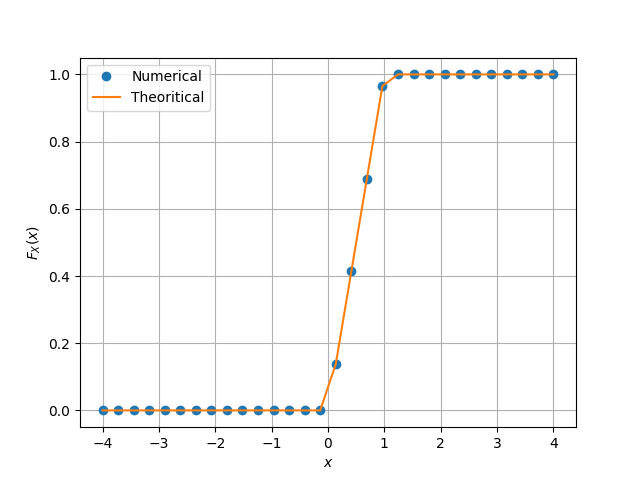
\includegraphics[width=\columnwidth]{figs/uni_cdf.png}
\caption{The CDF of $U$}
\label{fig:uni_cdf}
\end{figure}

%
\item
Find a theoretical expression for $F_{U}(x)$.\\
\solution Given that, random variable $U$ is uniformly distributed in interval $\brak{0,1}$ . So we can write that, the probability density function
               \begin{align}
                        f_{U}\brak{x} &= \frac{1}{1 -0}\\
                                      &= 1
               \end{align}
       So for $ x \in \brak{0,1} $,the probability distribution function $F_{U}\brak{x}$ can be calculated as,
               \begin{align}
                           F_{U}\brak{x} &= \int_{0}^{x} f_x\brak{x}dx\\
                                         &= \int_{0}^{x}1dx\\
                                         &= x
                \end{align}

       For $x<0$,
		\begin{align}
			F_{U}\brak{x} &= \pr{U \leq x}
				      &= 0 \brak{\because f_{U}\brak{x} = 0}
                \end{align}
	And for $x>1$
		\begin{align}
			F_{U}\brak{x} &= \pr{U \leq x}
			&= 1 \brak{\because f_{U}\brak{x} = 0}
    \end{align}
        Overall,		
		\begin{equation*}
			F_{U}\brak{x} = \begin{cases}      \label{cdf_U}
                                                          0  &, x \leq 0 \\
                                                          x  &, 0<x<1 \\
                                                          1  & , x \geq 1
                                                        \end{cases}
                 \end{equation*}

\item
The mean of $U$ is defined as
%
\begin{equation}
E\sbrak{U} = \frac{1}{N}\sum_{i=1}^{N}U_i
\end{equation}
%
and its variance as
%
\begin{equation}
\text{var}\sbrak{U} = E\sbrak{U- E\sbrak{U}}^2 
\end{equation}

Write a C program to  find the mean and variance of $U$.\\ 
\solution Download the following code,
 \begin{lstlisting}
wget https://github.com/Charanyash/Random-Numbers-/blob/main/codes/Q1/mean_var_uniform.c
wget https://github.com/Charanyash/Random-Numbers-/blob/main/codes/Q1/coeffs.h
 \end{lstlisting}
Run the following command,
 \begin{lstlisting}
cc mean_var_uniform.c -lm
./a.out
 \end{lstlisting}
We will get output as,
\begin{align}
	mean &= 0.500007\\
  variance&= 0.083301
\end{align}
	
\item Verify your result theoretically given that
\end{enumerate}
%
\begin{equation}
E\sbrak{U^k} = \int_{-\infty}^{\infty}x^kdF_{U}(x)
\end{equation}
\solution Already we know that,
                \begin{equation*}
                                 F_{U}\brak{x} = \begin{cases} \label{cdf_U}
                                                          0  &, x \leq 0 \\
                                                          x  &, 0<x<1 \\
                                                          1  & , x \geq 1
                                                        \end{cases}
                 \end{equation*}

So, the given integral solves down to,
 \begin{equation}
	 E\sbrak{U^k} = \int_{0}^{1}x^kdx
 \end{equation}
Since $F_{U}\brak{x}$ is constant w.r.t x for $ x \geq 1 $ amd $ x \leq 0 $.\\
For mean,
  \begin{align}
	  E\sbrak{U} &= \int_{0}^{1}xdx\\
	             &=\cbrak{ \frac{x^{2}}{2}}_{0}^{1}\\ 
                     &= 0.5
  \end{align}
Now for variance,we know that
  \begin{align}
	  Var\sbrak{U} &= E\sbrak{U- E\sbrak{U}}^2 \\
		       &= E\sbrak{U^{2} + E\sbrak{U}^{2} - 2E\sbrak{U}U}\\
  \end{align}
  Since expected value is a linear operator, we can write
  \begin{align}
	               &= E\sbrak{U^{2}} + E\sbrak{U}^{2} - 2E\sbrak{U}^{2}\\
                   &= E\sbrak{U^{2}} - E\sbrak{U}^{2} \label{eq:1-8}
  \end{align}
 To get variance we will find,
  \begin{align}
	  E\sbrak{U^{2}} &= \int_{0}^{1}x^{2}dx\\
			 &=\cbrak{ x^{3}/3}_{0}^{1}\\
			 &= \frac{1}{3}
  \end{align}
  Therefore,
  \begin{align}
	  Var\sbrak{U} &= \frac{1}{3} -\brak{\frac{1}{2}}^{2}\\
		       &= \frac{1}{3} - \frac{1}{4}\\
		       &= \frac{1}{12}\\
		       &= 0.0833
  \end{align}
\section{Central Limit Theorem}
%
\begin{enumerate}[label=\thesection.\arabic*
,ref=\thesection.\theenumi]

%
\item
Generate $10^6$ samples of the random variable
%
\begin{equation}
X = \sum_{i=1}^{12}U_i -6
\end{equation}
%
using a C program, where $U_i, i = 1,2,\dots, 12$ are  a set of independent uniform random variables between 0 and 1
and save in a file called gau.dat.\\
\solution Download the code below
\begin{lstlisting}
wget https://github.com/Charanyash/Random-Numbers-/blob/main/codes/Q2/gaussian.c
wget https://github.com/Charanyash/Random-Numbers-/blob/main/codes/Q2/coeffs.h
\end{lstlisting}
Run the following command
\begin{lstlisting}
cc  gaussian.c
./a.out
\end{lstlisting}
%
\item
Load gau.dat in python and plot the empirical CDF of $X$ using the samples in gau.dat. What properties does a CDF have?\\
\solution Download the below code,
\begin{lstlisting}
wget https://github.com/Charanyash/Random-Numbers-/blob/main/codes/Q2/gaussian_cdf_plot.py
\end{lstlisting}
Run the following command to get CDF plot,
\begin{lstlisting}
python3 gaussian_cdf_plot.py
\end{lstlisting}
The CDF of $X$ is plotted in Fig. \ref{fig:gauss_cdf}.\\
\textbf{Properties Of CDF:}
 \begin{itemize}
      \item CDF is montonically increasing from $ -\infty < x< \infty$	 
      \item Let us define the $Q\brak{x}$ function as,\\
	      $ Q\brak{x} = \pr{X>x} $
      \item The CDF,$F_{X}\brak{x} = 1-Q\brak{x} =Q\brak{-x} $ 	      
 \end{itemize}

\begin{figure}
\centering
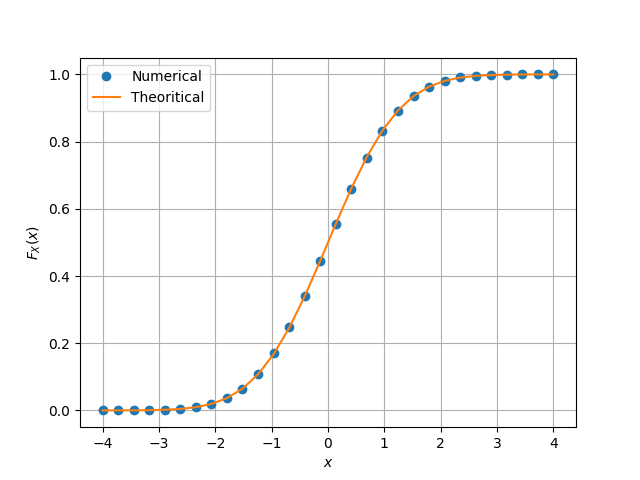
\includegraphics[width=\columnwidth]{figs/gauss_cdf.png}
\caption{The CDF of $X$}
\label{fig:gauss_cdf}
\end{figure}

\item
Load gau.dat in python and plot the empirical PDF of $X$ using the samples in gau.dat. The PDF of $X$ is defined as
\begin{align}
p_{X}(x) = \frac{d}{dx}F_{X}(x)
\end{align}
What properties does the PDF have?\\
\solution The PDF of $X$ is plotted in Fig. \ref{fig:gauss_pdf} using the code below
\begin{lstlisting}
wget https://github.com/Charanyash/Random-Numbers-/blob/main/codes/Q2/gaussian_pdf_plot.py
\end{lstlisting}
Run the following command,
\begin{lstlisting}
python3 gaussian_pdf_plot.py
\end{lstlisting}
\textbf{Properties of PDF:}
 \begin{enumerate}
 	 \item $\forall x \in \mathbb{R}$, $p_X(x) \geq 0$
     \item PDF is symmetric about the mean, in this case at $x=0$
     \item The maxima of the curve is observed at mean of distribution.
 \end{enumerate}	     

\begin{figure}
\centering
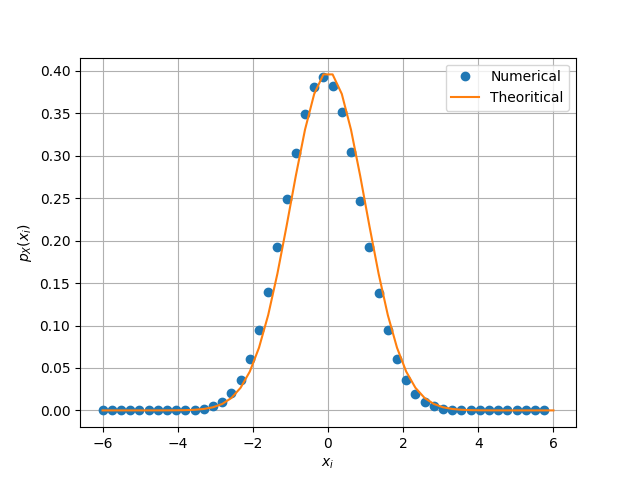
\includegraphics[width=\columnwidth]{figs/gauss_pdf.png}
\caption{The PDF of $X$}
\label{fig:gauss_pdf}
\end{figure}

\item Find the mean and variance of $X$ by writing a C program.\\
\solution Download the C code from the links below,
\begin{lstlisting}
wget https://github.com/Charanyash/Random-Numbers-/blob/main/codes/Q2/mean_var_gauss.c
wget https://github.com/Charanyash/Random-Numbers-/blob/main/codes/Q2/coeffs.h
\end{lstlisting}
Then run the following command in linux terminal
\begin{lstlisting}
cc mean_var_gauss.c -lm
./a.out
\end{lstlisting}
we will get $mean = 0.000326, variance = 1.000906$
\item Given that 
\begin{align}
p_{X}(x) &= \frac{1}{\sqrt{2\pi}}\exp\brak{-\frac{x^2}{2}}, -\infty < x < \infty,
\end{align}
repeat the above exercise theoretically.\\
\solution Given that,
 \begin{align}
p_{X}(x) &= \frac{1}{\sqrt{2\pi}}\exp\brak{-\frac{x^2}{2}}, -\infty < x < \infty,
 \end{align} 
 We know,
   \begin{align}
	   E\sbrak{x} &= \int_{-\infty}^{\infty}xp_{X}\sbrak{x}dx\\
	              &= \int_{-\infty}^{\infty}\frac{1}{\sqrt{2\pi}}x\exp\brak{-\frac{x^2}{2}}dx
   \end{align}
 Since $\frac{1}{\sqrt{2\pi}}x\exp\brak{-\frac{x^2}{2}}$ is an odd function.We can write,
   \begin{align}
	   E\sbrak{x} &= 0 \label{eq:2-3}
   \end{align}
 Consider the following expression,
   \begin{align}
	   E\sbrak{x^{2}} &= \int_{-\infty}^{\infty}x^{2}p_{X}\sbrak{x}dx\\
	                  &=\frac{1}{\sqrt{2\pi}}\int_{-\infty}^{\infty}x^{2}e^{\brak{-\frac{x^2}{2}}}dx
   \end{align}
To solve the above integral, we will use integration by parts, i.e,\\
  \begin{align}
	  \int uvdx &= u\int vdx -\int u'\brak{\int vdx}dx  \\
	  E\sbrak{x^{2}} &= \frac{1}{\sqrt{2\pi}}\int_{-\infty}^{\infty}x\brak{xe^{-\frac{x^2}{2}}}dx\\
			         &= \frac{1}{\sqrt{2\pi}}\brak{x\int x e^{-\frac{x^2}{2}}dx -  \int\brak{\int xe^{-\frac{x^2}{2}}dx}}
  \end{align}
For the integral $\int x\exp\brak{-\frac{x^2}{2}}dx$ let us take,
  \begin{align}
	   t &= \frac{x^2}{2}\\
	  dt &= xdx\\
	  \int x\exp\brak{-\frac{x^2}{2}}dx &= \int\exp\brak{-t}dt\\
					                    &=  -\exp\brak{-t} + c \\
				 \implies  &= -\exp\brak{-\frac{x^{2}}{2}} + c \label{eq:2-6}
  \end{align}
 Using \eqref{eq:2-6},we can write
  \begin{align}
	  E\sbrak{x^{2}} &= \frac{1}{\sqrt{2\pi}}\brak{ -xe^{-\frac{x^{2}}{2}} + \int e^{\frac{-x^{2}}{2}}dx}
  \end{align}
  And we know that,
  \begin{align}
	  \frac{1}{\sqrt{2\pi}}\int_{-\infty}^{\infty}e^{\frac{-x^{2}}{2}} &= 1 \label{eq:2-8}
  \end{align}
 Now putting limits and using \eqref{eq:2-3},\eqref{eq:2-8},
  \begin{align}
     E\sbrak{x^{2}} &= 1
  \end{align}	  
Using \eqref{eq:1-8} we can write,
   \begin{align}
    Var\sbrak{x} &= 1 - 0\\
	         &= 1
   \end{align}                           
%
\end{enumerate}
\section{From Uniform to Other}
\begin{enumerate}[label=\thesection.\arabic*,ref=\thesection.\theenumi]
%
\item
Generate samples of 
%
\begin{equation}
V = -2\ln\brak{1-U}
\end{equation}
%
and plot its CDF.\\
\solution Download the C code from the link below to generate samples of V from uni.dat file
\begin{lstlisting}
wget  https://github.com/Charanyash/Random-Numbers-/blob/main/codes/Q3/V.c
\end{lstlisting}
Run the following command,
\begin{lstlisting}
cc V.c -lm
./a.out
\end{lstlisting}
Then download the below python file to get CDF
\begin{lstlisting}
wget https://github.com/Charanyash/Random-Numbers-/blob/main/codes/Q3/V_cdf_plot.py
\end{lstlisting}
Then run the following command
\begin{lstlisting}
python3 V_cdf_plot.py
\end{lstlisting}
\begin{figure}
\centering
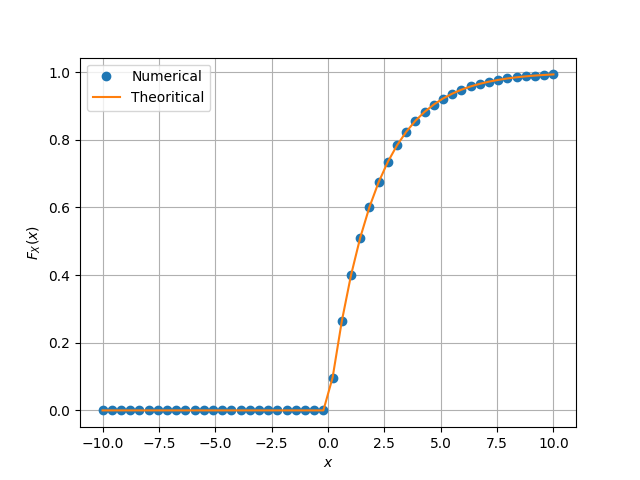
\includegraphics[width=\columnwidth]{figs/V_cdf.png}
\caption{The CDF of $V$}
\label{fig:V_cdf}
\end{figure}
\item Find a theoretical expression for $F_V(x)$.\\
\solution Given 
\begin{align}
	V &= -2\ln\brak{1-U}\\ \label{eq: 3-2}
	 F_V\brak{x} &= \pr{V\leq x}
\end{align}
 we will use \eqref{eq: 3-2}
 \begin{align}
	 F_V\brak{x} &= \pr{-2\ln\brak{1-U} \leq x}\\
	             &= \pr{ \ln\brak{1-U} \geq \frac{-x}{2}}\\
		         &= \pr{  1-U \geq \exp\brak{\frac{-x}{2}}}\\
		         &= \pr{ U \leq 1 - \exp\brak{\frac{-x}{2}}}\\
                 &= F_U\brak{1-\exp\brak{\frac{-x}{2}}}
 \end{align}
  For$ x > 0, 1 - e^{\frac{-x}{2}} < 1$ and $x<0 , 1 - e^{\frac{-x}{2}} < 0 $ 		
 \begin{align}
	 F_V\brak{x} &=
	           \begin{cases}
			                0  & x\leq 0 \\
		            1-\exp\brak{\frac{-x}{2}} & x >0	   
                   \end{cases}
 \end{align}		   
%
%\item
%Generate the Rayleigh distribution from Uniform. Verify your result through graphical plots.
 \section{Triangular Distribution}
\begin{enumerate}[label=\thesection.\arabic*
,ref=\thesection.\theenumi]
%
\item Generate
	\begin{align}
		T = U_1+U_2
	\end{align}
\solution Download the below code,
 \begin{lstlisting}
 wget https://github.com/Charanyash/Random-Numbers-/blob/main/codes/Q4/coeffs.h
 wget https://github.com/Charanyash/Random-Numbers-/blob/main/codes/Q4/triangular.c
 \end{lstlisting}
and run the following command,
 \begin{lstlisting}
  cc triangular.c -lm
  ./a.out
 \end{lstlisting}
 You will get required generated random numbers in tri.dat file.		
\item Find the CDF of $T$.\\
 \solution Download the below files,
  \begin{lstlisting}
   wget https://github.com/Charanyash/Random-Numbers-/blob/main/codes/Q4/tri.dat
   wget https://github.com/Charanyash/Random-Numbers-/blob/main/codes/Q4/tri_cdf_plot.py
  \end{lstlisting}
  Run the following command,
  \begin{lstlisting}
   python3 tri_cdf_plot.py
  \end{lstlisting}
  \begin{figure}
   \centering
   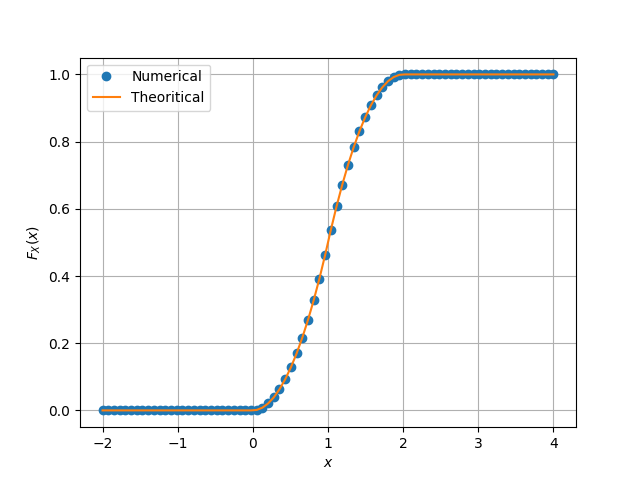
\includegraphics[width=\columnwidth]{Q4/tri_cdf.png}
   \caption{The CDF of $T$}
   \label{fig:tri_cdf}
  \end{figure}
\item Find the PDF of $T$.\\
 \solution Download the below files,
  \begin{lstlisting}
   wget https://github.com/Charanyash/Random-Numbers-/blob/main/codes/Q4/tri.dat
   wget https://github.com/Charanyash/Random-Numbers-/blob/main/codes/Q4/tri_pdf_plot.py
  \end{lstlisting}
  Run the following command,
  \begin{lstlisting}
   python3 tri_pdf_plot.py
  \end{lstlisting}		
 \begin{figure}
  \centering
  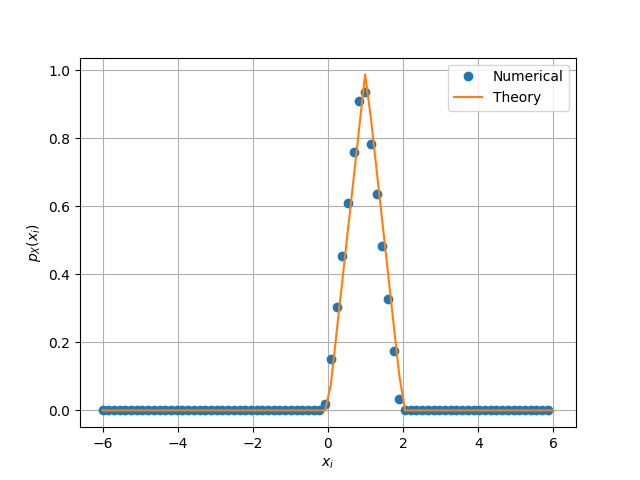
\includegraphics[width=\columnwidth]{Q4/tri_pdf.png}
  \caption{The PDF of $T$}
  \label{fig:tri_pdf}
 \end{figure}
\item Find the theoretical expressions for the PDF and CDF of $T$.\\
  \solution Given that,
   \begin{align}
           T = U1 + U2 \label{eq 4-1} 
   \end{align}
where$ U1, U2 $ are uniform random variables $\in \brak{0,1}$.\\
The CDF of T is defined as,
   \begin{align}
            F_{T}\brak{t} &= \pr{T \leq t}
   \end{align}
  Now from $\eqref{eq 4-1}$ we can write,
   \begin{align}
           F_{T}\brak{t}  &= \pr{U1 + U2 \leq t}
   \end{align}
 \textbf{Case -1 :} For $ t> 2$.\\
  The $\pr{ U1 + U2 \leq t} = 1$, because for every $ U1 = u1$ and $U2 = u2$, $u1 + u2 <2$,
   \begin{align}
           \implies F_{T}\brak{t} &= 1 
   \end{align}
 \textbf{Case -2 :} For $ t<0$.\\
  The $\pr{ U1 + U2 \leq t} = 0$ because for every $ U1 = u1$ and $U2 = u2$, $u1 + u2 >0$,
   \begin{align}
           \implies F_{T}\brak{t} &= 0 
   \end{align}
 \textbf{Case - 3:} For, $ t \in \brak{0,2} $.\\
  We cannot eliminate the inequality like we did before, so in this case we will operate the inequality by fixing $U1 = x$ where $x\in \brak{0,t} $. So in this case CDF will be,
   \begin{align}
           F_{T}\brak{t}  &= \pr{U1 + U2 \leq t}\\
                          &= \pr{U1 = x,U2 \leq t-x}\\
                          &= \pr{U1 = x}\pr{U2 \leq t-x}  
   \end{align}
 Since U1,U2 are i.i.d.\\
  Now note that $ x$ is a variable and varies in $\brak{0,t}$ , so we have to take integral over x to evaluate the $\pr{U1=x}$ ,
   \begin{align}
           F_{T}\brak{t} &= \int_{0}^{t} f_{U}\brak{x}\pr{U2 \leq t-x} dx\\
                         & =\int_{0}^{t} f_{U}\brak{x}F_{U}\brak{t-x} dx
   \end{align}
\textbf{Case - 1} For $ t \in \brak{0,1} $,we know $f_{U}\brak{x} = 1$ so,
  \begin{align}
          F_{T}\brak{t} &= \int_{0}^{t}1.F_{U}\brak{t-x}dx
  \end{align}
        As, $x<t$ , $ 0<t-x< t<1$ using \eqref{cdf_U},we can write
  \begin{align}
         F_{T}\brak{t} &= \int_{0}^{t}\brak{t-x}dx\\
                       &= \cbrak{ tx - \frac{x^2}{2}}_{0}^{t}\\
                       &= \frac{t^{2}}{2}
  \end{align}
 \textbf{Case -2} For $ t \in \brak{1,2}$ , we know $f_{U}\brak{x} = 0$ at $ x > 1$ ,so the integral solves down to,
  \begin{align}
          F_{T}\brak{t} &= \int_{0}^{1}f_{U}\brak{x}F_{U}\brak{t-x}dx\\
                        &= \int_{0}^{1}1.F_{U}\brak{t-x}dx\\
  \end{align}
   To solve the above integral we will use integration by substitution,
   \begin{align}
            k &= t-x\\
           dk &= -dx\\
           F_{T}\brak{t} &= \int_{t}^{t-1}F_{U}\brak{k}\brak{-dk}\\
                         &= \int_{t-1}^{t}F_{U}\brak{k}dk
   \end{align}
   As $ 1 \leq t \leq 2 , 0 \leq t-1 \leq 1 $ we will break integral at 1 because $ F_{U}\brak{k}$ changes at 1.Using \eqref{cdf_U},
   \begin{align}
           F_{T}\brak{t}  &= \int_{t-1}^{1}F_{U}\brak{k}dk + \int_{1}^{t}F_{U}\brak{k}dk \\
                          &= \int_{t-1}^{1}kdk + \int_{1}^{t}1dk\\
                          &= \cbrak{\frac{k^{2}}{2}}_{t-1}^{1} + t - 1\\
                          &= \frac{1}{2} -\brak{\frac{\brak{t-1}^{2}}{2}} + t - 1\\
                          &= 2t - \frac{t^{2}}{2} - 1
   \end{align}
   Overall we can write the CDF of $F_{T}\brak{x}$ as,
   \begin{align}
           F_{T}\brak{x} &=   \begin{cases}
                                   0                      &,   x <0\\
                                \frac{x^{2}}{2}           &, 0\leq x \leq 1\\
                                2t - \frac{t^{2}}{2} - 1  &, 1 \leq x \leq 2\\
                                   1                      &,   x > 2
                              \end{cases}
    \end{align}                      
 Now we will find PDF of $T$,\\
 As,
   \begin{align}
           T &= U1 + U2
   \end{align}
  We will use method of convolution to get PDF of $T$ as $ U1$ and $U2$ are i.i.d.
   \begin{align}
          f_{T}\brak{t} &= \int_{-\infty}^{\infty}f_{U1}\brak{x}f_{U2}\brak{t-x}dx
   \end{align}
  Since $ U1,U2$ are of same distribution we can write,
   \begin{align}
           f_{U1}\brak{x} &= f_{U2}\brak{x} = f_{U}\brak{x}\\
           \implies f_{T}\brak{t} &= \int_{-\infty}^{\infty}f_{U}\brak{x}f_{U}\brak{t-x}dx
   \end{align}
 From the PDF of U,we can write
  \begin{align}
          f_{T}\brak{t} &= \int_{0}^{1}f_{U}\brak{x}f_{U}\brak{t-x}dx\\
                        &= \int_{0}^{1}1.f_{U}\brak{t-x}dx\\
  \end{align}
  we will solve the above integral using substitution.
  \begin{align}
            z &= t-x \\
           dz &= -dx \\
          \implies f_{T}\brak{t} &= \int_{t}^{t-1}f_{U}\brak{z}\brak{-dz}\\
                                 &= \int_{t-1}^{t}f_{U}\brak{z}dz
  \end{align}
 \textbf{Case -1} For $ t<0 $ as $ z <t $,the PDF $ f_{U}\brak{z} = 0 $. So,
  \begin{align}
          f_{T}\brak{t} &= 0
  \end{align}
 \textbf{Case -2} For $ 0 \leq t \leq 1$, we will break the integral at $z = 0$, since $f_{U}\brak{z}$ changes at 0.
  \begin{align}
          f_{T}\brak{t} &= \int_{t-1}^{0}f_{U}\brak{z}dz + \int_{0}^{t}f_{U}\brak{z}dz\\
                        &= 0 + \int_{0}^{t}1dz \\
                        &= t
  \end{align}
 \textbf{Case-3} Similarly for $ 1 \leq t \leq 2$, we will break the integral at $ z = 1 $,
  \begin{align}
          f_{T}\brak{t} &= \int_{t-1}^{1}f_{U}\brak{z}dz + \int_{1}^{t}f_{U}\brak{z}\\
                        &= \int_{t-1}^{1}1.dz + 0\\
                        &=  2 - t
  \end{align}
   \textbf{Case-4} For $ t>2$,as $ z > t - 1  > 1$,the PDF $f_{U}\brak{z} = 0 $. So,
   \begin{align}
           f_{T}\brak{z} &= 0
   \end{align}
  Overall, the PDF of T will be,
   \begin{align}
           f_{T}\brak{x} &=  \begin{cases}
                                     0     &, x <0 \\
                                     x     &, 0 \leq x \leq 1\\
                                    2-x    &, 1 \leq x \leq 2 \\
                                     0     &, x > 2
                             \end{cases}
   \end{align}
\item Verify your results through a plot.\\
  \solution This is already done in \ref{fig:tri_cdf} ,\ref{fig:tri_pdf}.
\end{enumerate}
\section{Maximum Likelihood}
\begin{enumerate}[label=\thesection.\arabic*
,ref=\thesection.\theenumi]
\item Generate equiprobable $X \in \cbrak{1,-1}$.
\item Generate
\begin{equation}
Y = AX+N,
\end{equation}
		where $A = 5$ dB,  and $N \sim \gauss{0}{1}$.
	\item Plot $Y$ using a scatter plot.
	\item Guess how to estimate $X$ from $Y$.
\item
\label{ml-ch4_sim}
Find
\begin{equation}
	P_{e|0} = \pr{\hat{X} = -1|X=1}
\end{equation}
and
\begin{equation}
	P_{e|1} = \pr{\hat{X} = 1|X=-1}
\end{equation}
%
\item Find $P_e$ assuming that $X$ has equiprobable symbols.
%
\item
Verify by plotting  the theoretical $P_e$ with respect to $A$ from 0 to 10 dB.
%
\item Now, consider a threshold $\delta$  while estimating $X$ from $Y$. Find the value of $\delta$ that maximizes the theoretical $P_e$.
\item Repeat the above exercise when
	\begin{align}
		p_{X}(0) = p
	\end{align}
\item Repeat the above exercise using the MAP criterion.
		\end{enumerate}
\section{Gaussian to Other}
\begin{enumerate}[label=\thesection.\arabic*
,ref=\thesection.\theenumi]
\item
Let $X_1 \sim  \gauss{0}{1}$ and $X_2 \sim  \gauss{0}{1}$. Plot the CDF and PDF of
%
\begin{equation}
V = X_1^2 + X_2^2
\end{equation}
%
%
%
\item
If
%
\begin{equation}
F_{V}(x) =
\begin{cases}
1 - e^{-\alpha x} & x \geq 0 \\
0 & x < 0,
\end{cases}
\end{equation}
%
find $\alpha$.
%
\item
\label{ch3_raleigh_sim}
Plot the CDF and PDf of
%
\begin{equation}
A = \sqrt{V}
\end{equation}
%
\end{enumerate}
\section{Conditional Probability}
\begin{enumerate}[label=\thesection.\arabic*
,ref=\thesection.\theenumi]
\item
\label{ch4_sim}
Plot
\begin{equation}
P_e = \pr{\hat{X} = -1|X=1}
\end{equation}
%
for
\begin{equation}
Y = AX+N,
\end{equation}
where $A$ is Raleigh with $E\sbrak{A^2} = \gamma, N \sim \gauss{0}{1}, X \in \brak{-1,1}$ for $0 \le \gamma \le 10$ dB.
%
\item
Assuming that $N$ is a constant, find an expression for $P_e$.  Call this $P_e(N)$
%
\item
%
\label{ch4_anal}
For a function $g$,
\begin{equation}
E\sbrak{g(X)} = \int_{-\infty}^{\infty}g(x)p_{X}(x)\, dx
\end{equation}
%
Find $P_e = E\sbrak{P_e(N)}$.
%
\item
Plot $P_e$ in problems \ref{ch4_sim} and \ref{ch4_anal} on the same graph w.r.t $\gamma$.  Comment.
		\end{enumerate}
\section{Two Dimensions}
Let
\begin{equation}
\mbf{y} = A\mbf{x} + \mbf{n},
\end{equation}
where
\begin{align}
x &\in \brak{\mbf{s}_0,\mbf{s}_1},
\mbf{s}_0 =
\begin{pmatrix}
1
\\
0
\end{pmatrix},
\mbf{s}_1 =
\begin{pmatrix}
0
\\
1
\end{pmatrix}
\\
\mbf{n} &=
\begin{pmatrix}
n_1
\\
n_2
\end{pmatrix},
n_1,n_2 \sim \gauss{0}{1}.
\end{align}
%
\begin{enumerate}[label=\thesection.\arabic*
,ref=\thesection.\theenumi]
%%
\item
\label{ch5_fsk}
Plot
%
\begin{equation}
\mbf{y}|\mbf{s}_0 \text{ and } \mbf{y}|\mbf{s}_1
\end{equation}
%
on the same graph using a scatter plot.
%
\item
For the above problem, find a decision rule for detecting the symbols $\mbf{s}_0 $ and $\mbf{s}_1$.
%
\item
Plot
\begin{equation}
P_e = \pr{\hat{\mbf{x}} = \mbf{s}_1|\mbf{x} = \mbf{s}_0}
\end{equation}
with respect to the SNR from 0 to 10 dB.
%
\item
Obtain an expression for $P_e$. Verify this by comparing the theory and simulation plots on the same graph.
%
		\end{enumerate}
\end{enumerate}	
\end{document}
